  \subsection{Registration and Login System}
Every visitor who wants to use the application must register to the System.
After the registration, the Registered User must log into the System to use the mobile/web application.

\begin{table}[H]
	\centering
    
    \begin{tabular}{|p{3.5cm}|p{10.3cm}|}
    	\hline
    	\textbf{\large{Actors}} & 
		Visitor \\
    	& Registered User \\
	& Logged-In User \\
    \hline
    \textbf{\large{Goals}} 				& \ref{goal:trackme1} \ref{goal:trackme2}\\
    
    \hline
    \textbf{\large{Enter Condition}}	& There is no enter condition for this Use Case		\\
    
    \hline
    \textbf{\large{Events Flow}}		& \begin{enumerate}[leftmargin=0.5cm]
                                          	\item The \emph{Visitor}  accesses the web site or application sign-up page.
                                            \item The \emph{Visitor} inserts all the mandatory informations (username that will identify the user and password, personal data, email).
                                            \item The System registers the new Registered User and sends a confirmation email to the provided email address.
                                            \item The \emph{Visitor} becomes a \emph{Registered user} inserting a unique username and the password in the log in page.  
                                            \item The \emph{Registered User} now can access the \emph{TrackMe} services through the log in page.
                                            \item After the insertion of the identifier and password, the \emph{Registered User} becomes a \emph{Logged-in User}.
                                          \end{enumerate}
    										\\
    \hline
    \textbf{\large{Exit Condition}} 	& The User/Third Party is registered in the \emph{TrackMe} System, and his account is added to they system. Now the Registered User is able to use all the functionalities provided by the system. \\
    
    \hline
    \textbf{\large{Exception}} 			& \begin{enumerate}[leftmargin=0.5cm]
                                          	\item The \emph{Visitor} cannot register himself because he is already registered.
                                          	\item The \emph{Registered User} is not able to sign into the System because the login data are wrong or he did not confirm the registration.
                                            \end{enumerate}
    										If one of these problems occur, the system, both on the web site and on the mobile application, shows a message error to the User/Third Party, which is invited to re-insert their credentials or confirm the registration email.\\
    
    \hline
    
    \end{tabular}
	
\end{table}
\begin{figure}[H]

    \centering
    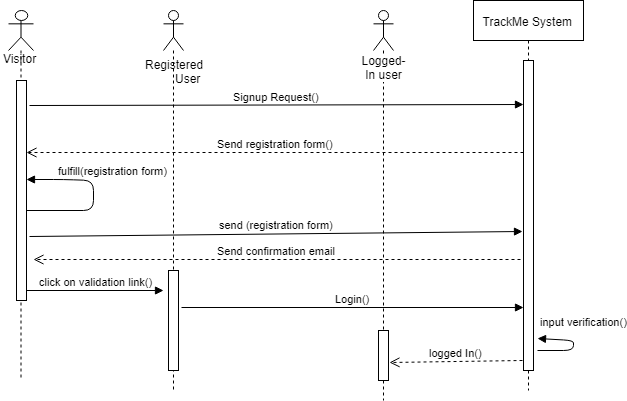
\includegraphics[scale=0.4]{./Pictures/login1.png}
    \caption{Sequence diagram for the registration and login process}
    
\end{figure}

